\subsection{تخمین پارامتر کانال‌های رول-پیچ}
برای اصلاح پارامترها رول-پیچ چندین آزمایش انجام شد و با استفاده از خروجی آزمایش و جعبه‌ابزاز
\lr{Parameter Estimator}
پارامترها اصلاح شدند.
برای آزمایش رول-پیچ تمامی موتورها با دور مختلف شروع به حرکت کردند و از خروجی سنسور داده برداری شد. سپس، مدل و  داده‌های ذخیره شده به جعبه‌ابزار
\lr{Parameter Estimator}
داده شد. نتایج آزمایش‌های کانال‌های رول-پیچ بعد از اصلاح پارامترها در شکل‌های
(\ref{roll_pitch_ps1}, \ref{roll_pitch_ps2}, \ref{roll_pitch_ps3}, \ref{roll_pitch_ps4}, \ref{roll_pitch_ps5}, \ref{roll_pitch_ps6}, \ref{roll_pitch_ps7})
آورده شده است.

\begin{figure}[H]
	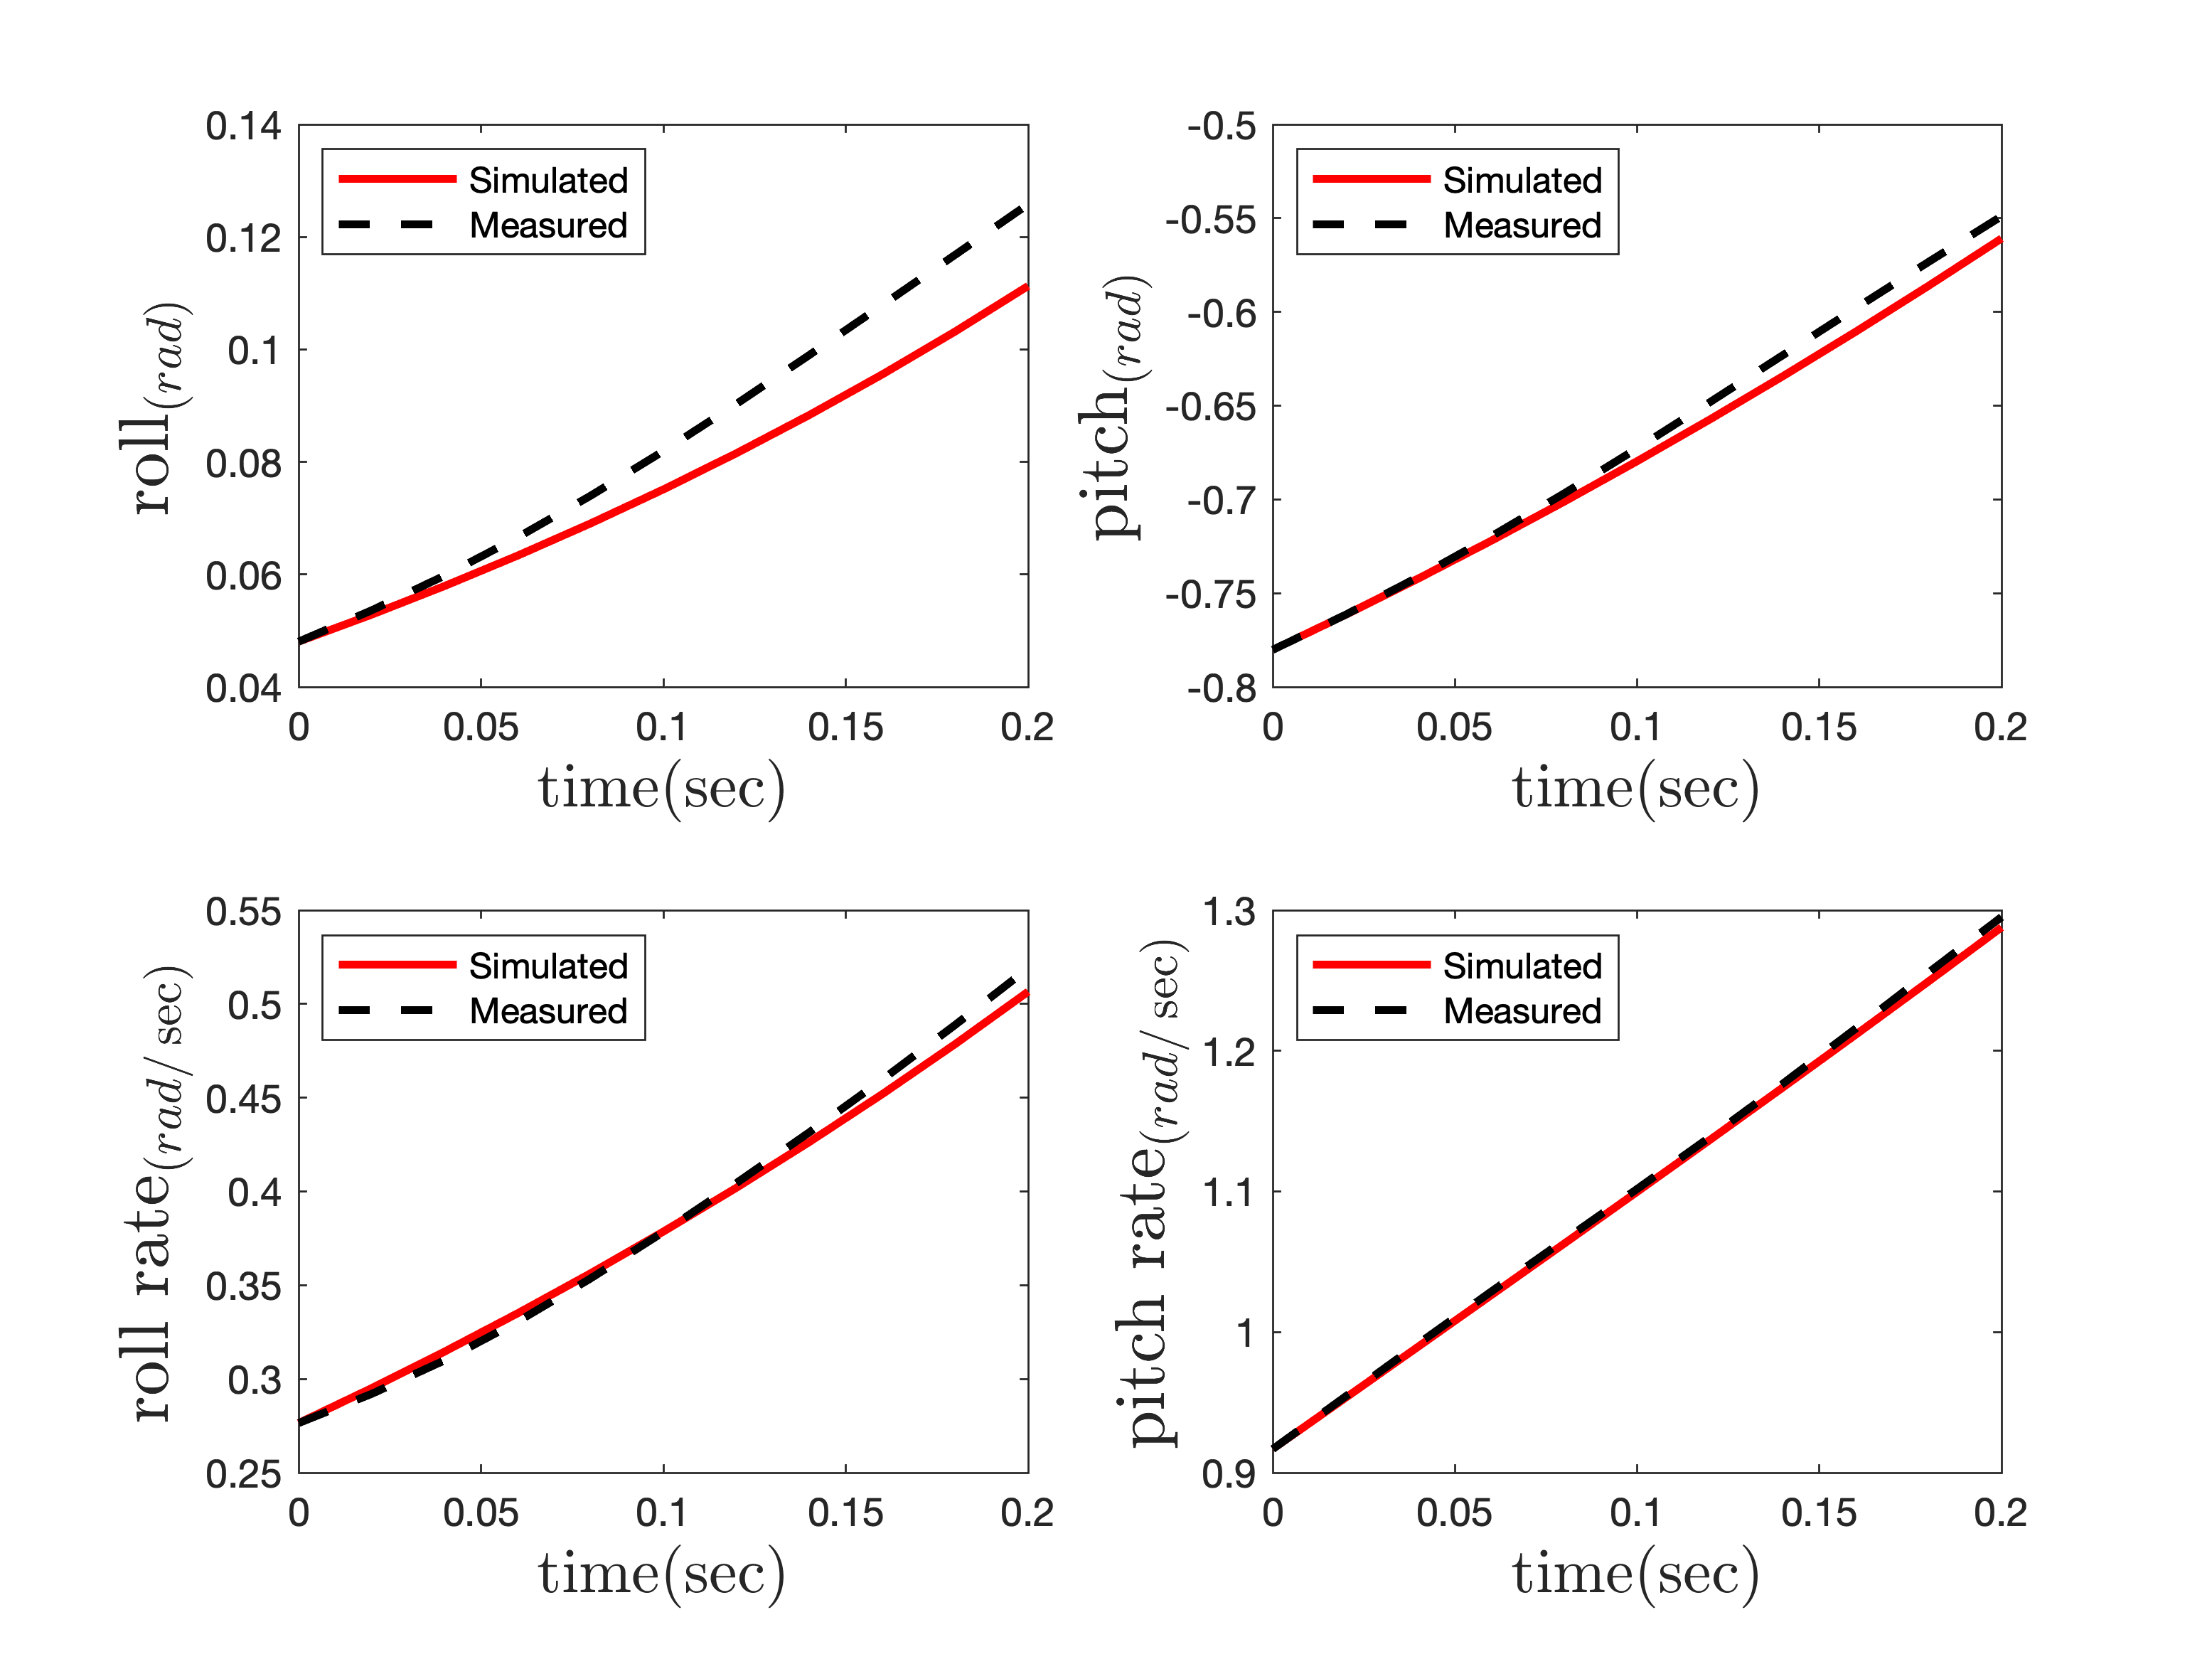
\includegraphics[width=12cm]{../../Figures/RCP/roll_pitch_parameter_estimation/RCP_roll_pitch_S1.png}
	\centering
	\caption{مقايسه خروجی‌های آزمايش اول و خروجی‌های شبیه‌سازی پس از تخمین پارامترهای کانال‌های رول-پیچ}
	\label{roll_pitch_ps1}
\end{figure}
\begin{figure}[H]
	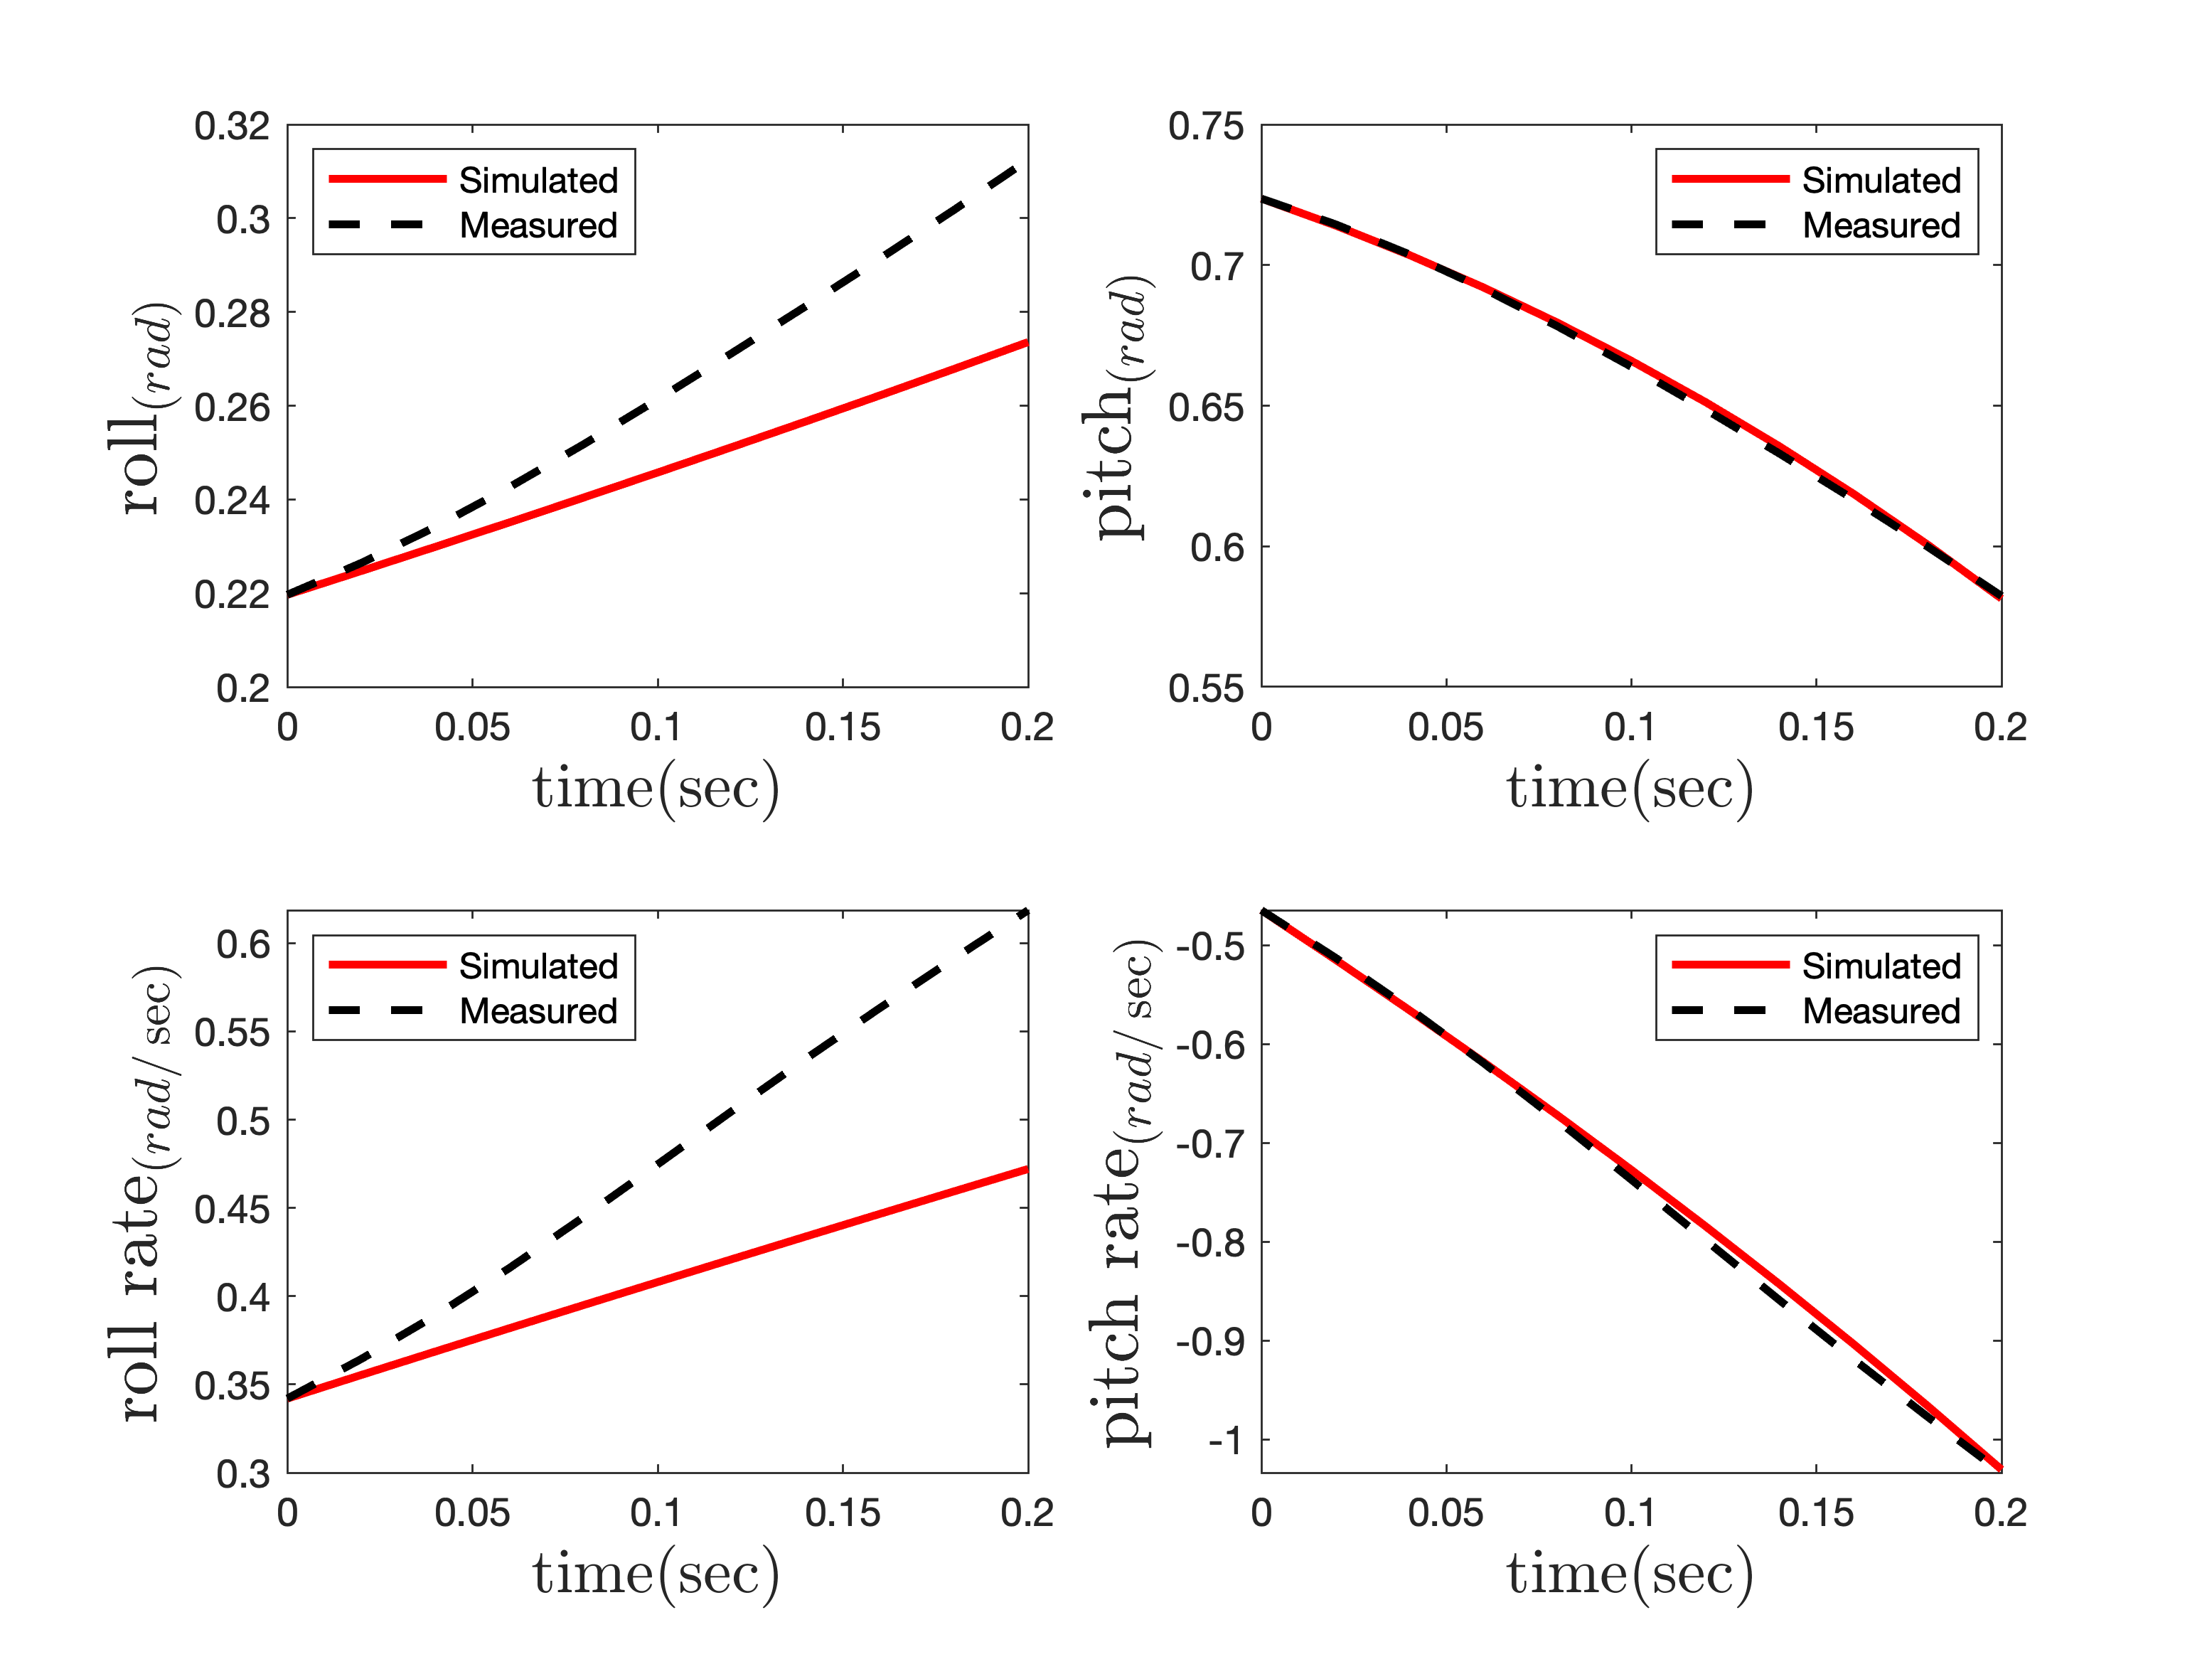
\includegraphics[width=12cm]{../../Figures/RCP/roll_pitch_parameter_estimation/RCP_roll_pitch_S2.png}
	\centering
	\caption{مقايسه خروجی‌های آزمايش دوم و خروجی‌های شبیه‌سازی پس از تخمین پارامترهای کانال‌های رول-پیچ}
	\label{roll_pitch_ps2}
\end{figure}
\begin{figure}[H]
	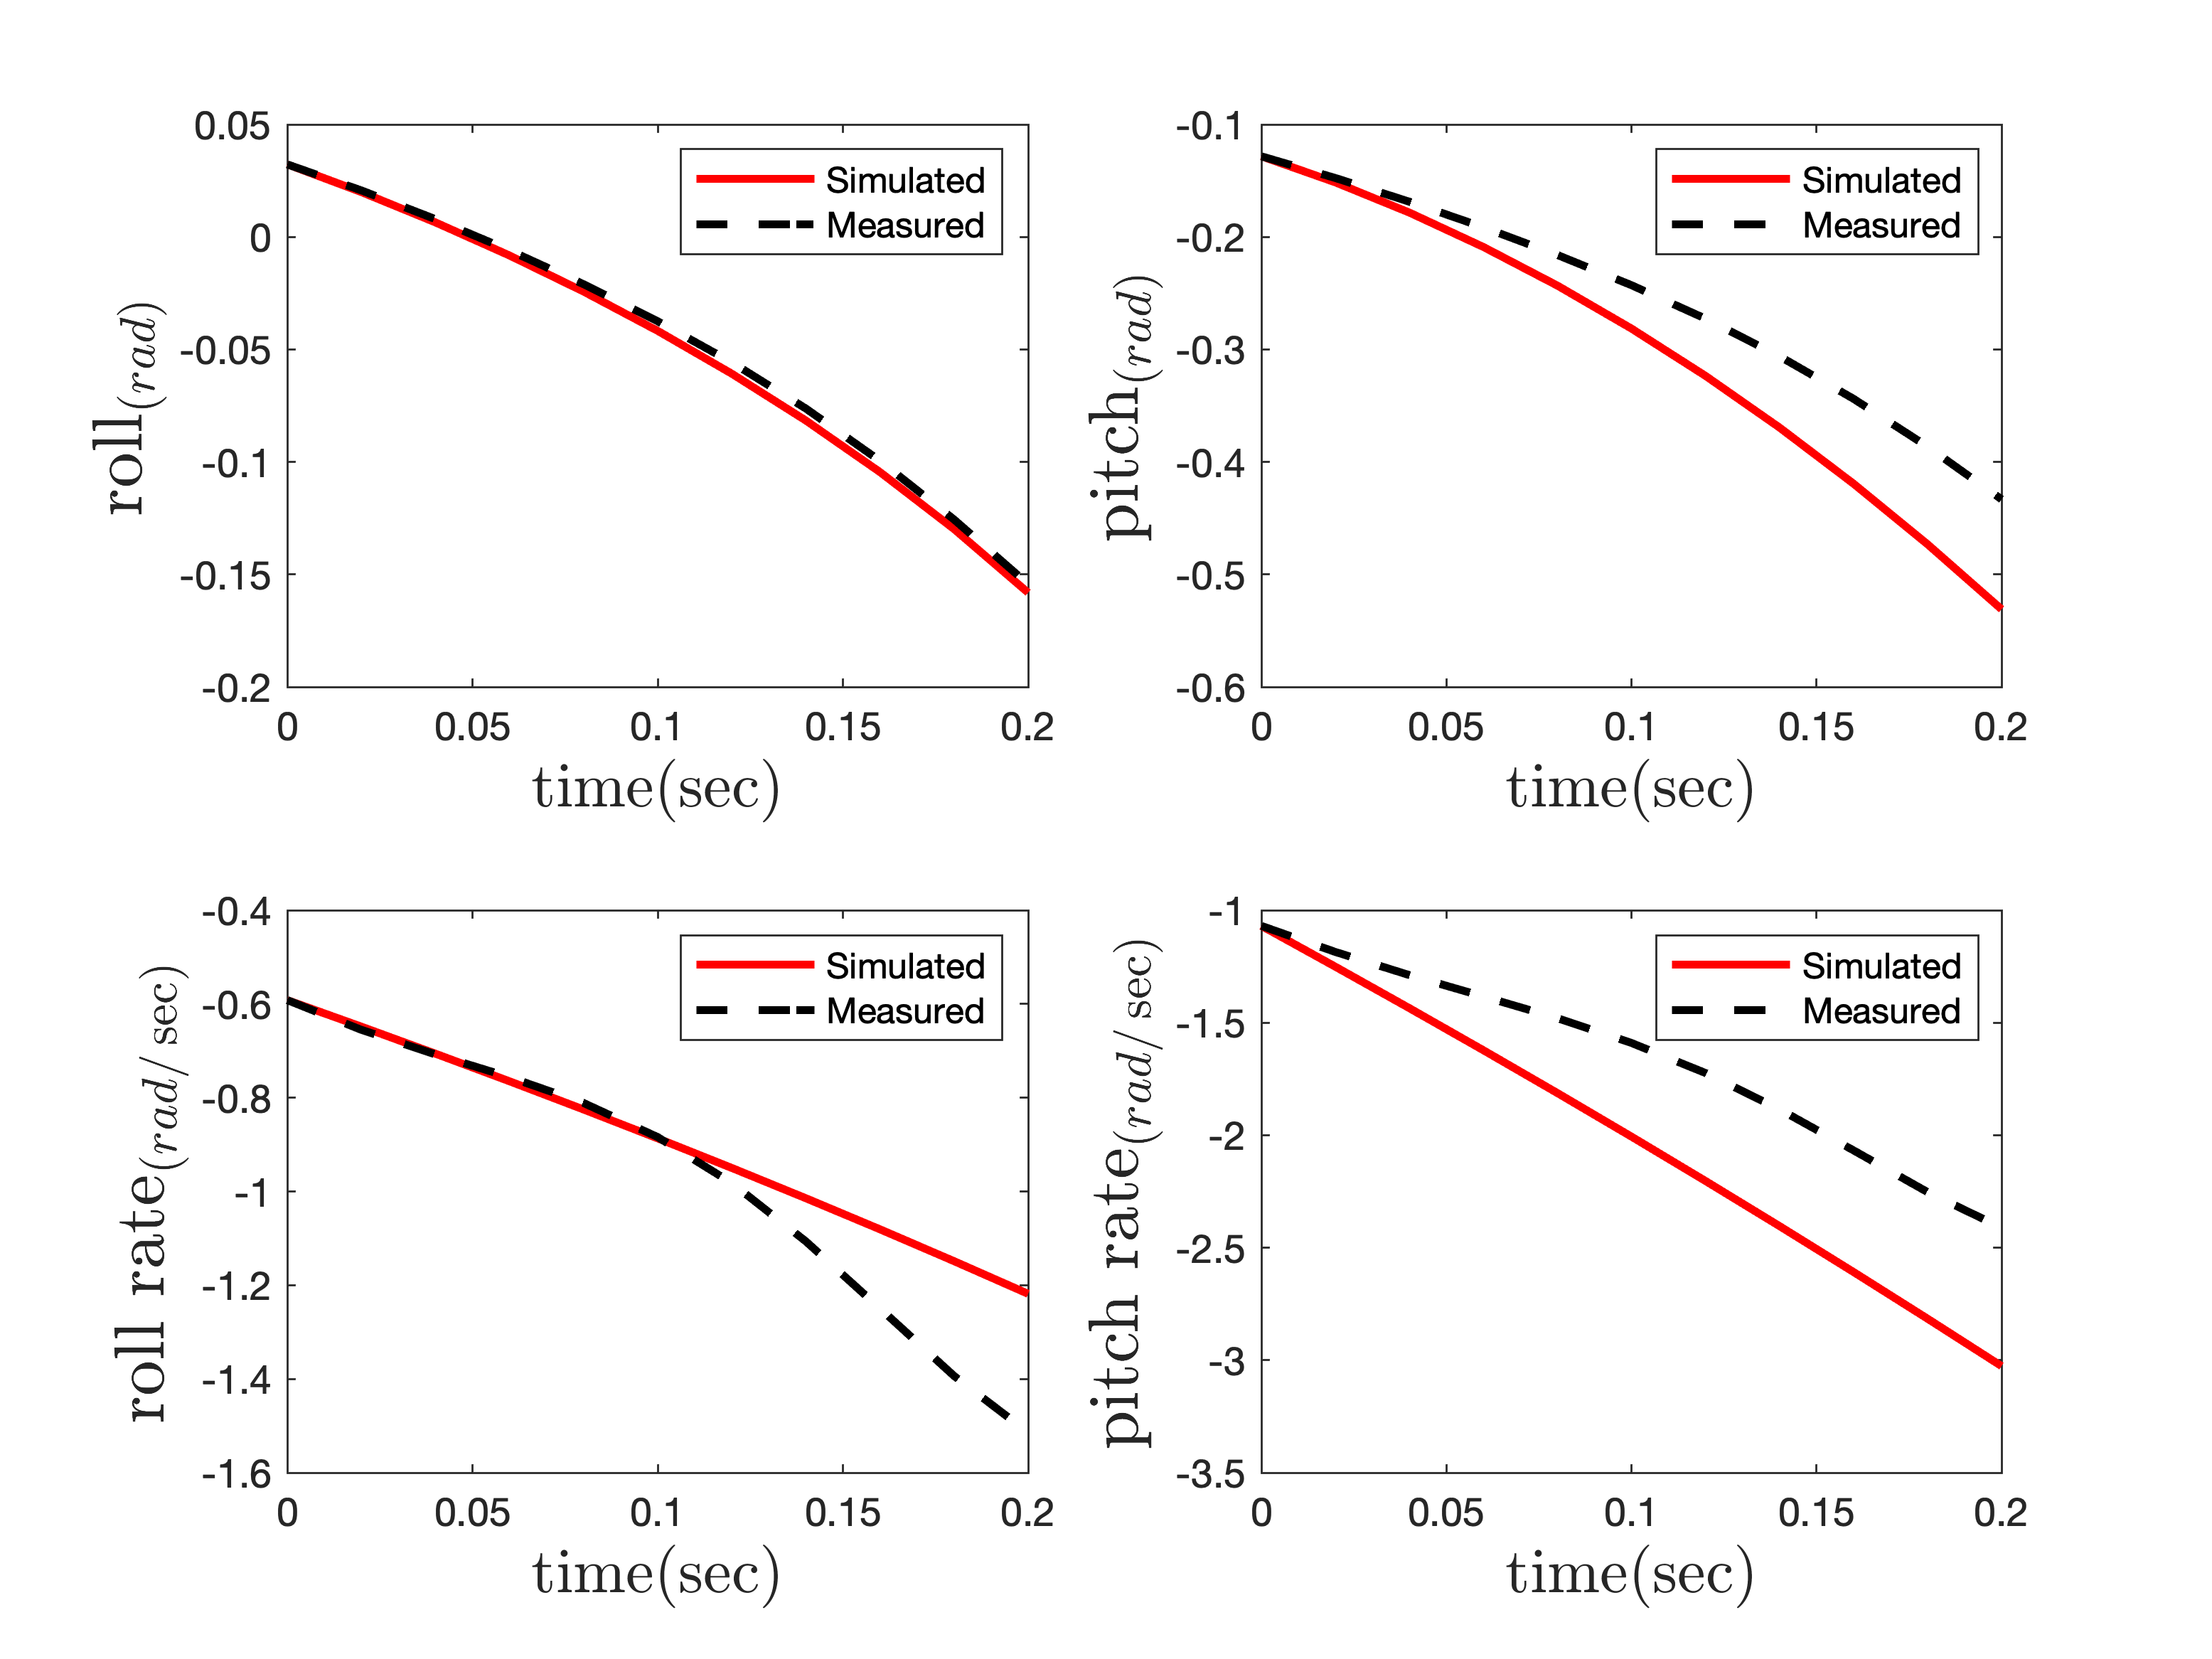
\includegraphics[width=12cm]{../../Figures/RCP/roll_pitch_parameter_estimation/RCP_roll_pitch_S3.png}
	\centering
	\caption{مقايسه خروجی‌های آزمايش سوم و خروجی‌های شبیه‌سازی پس از تخمین پارامترهای کانال‌های رول-پیچ}
	\label{roll_pitch_ps3}
\end{figure}
\begin{figure}[H]
	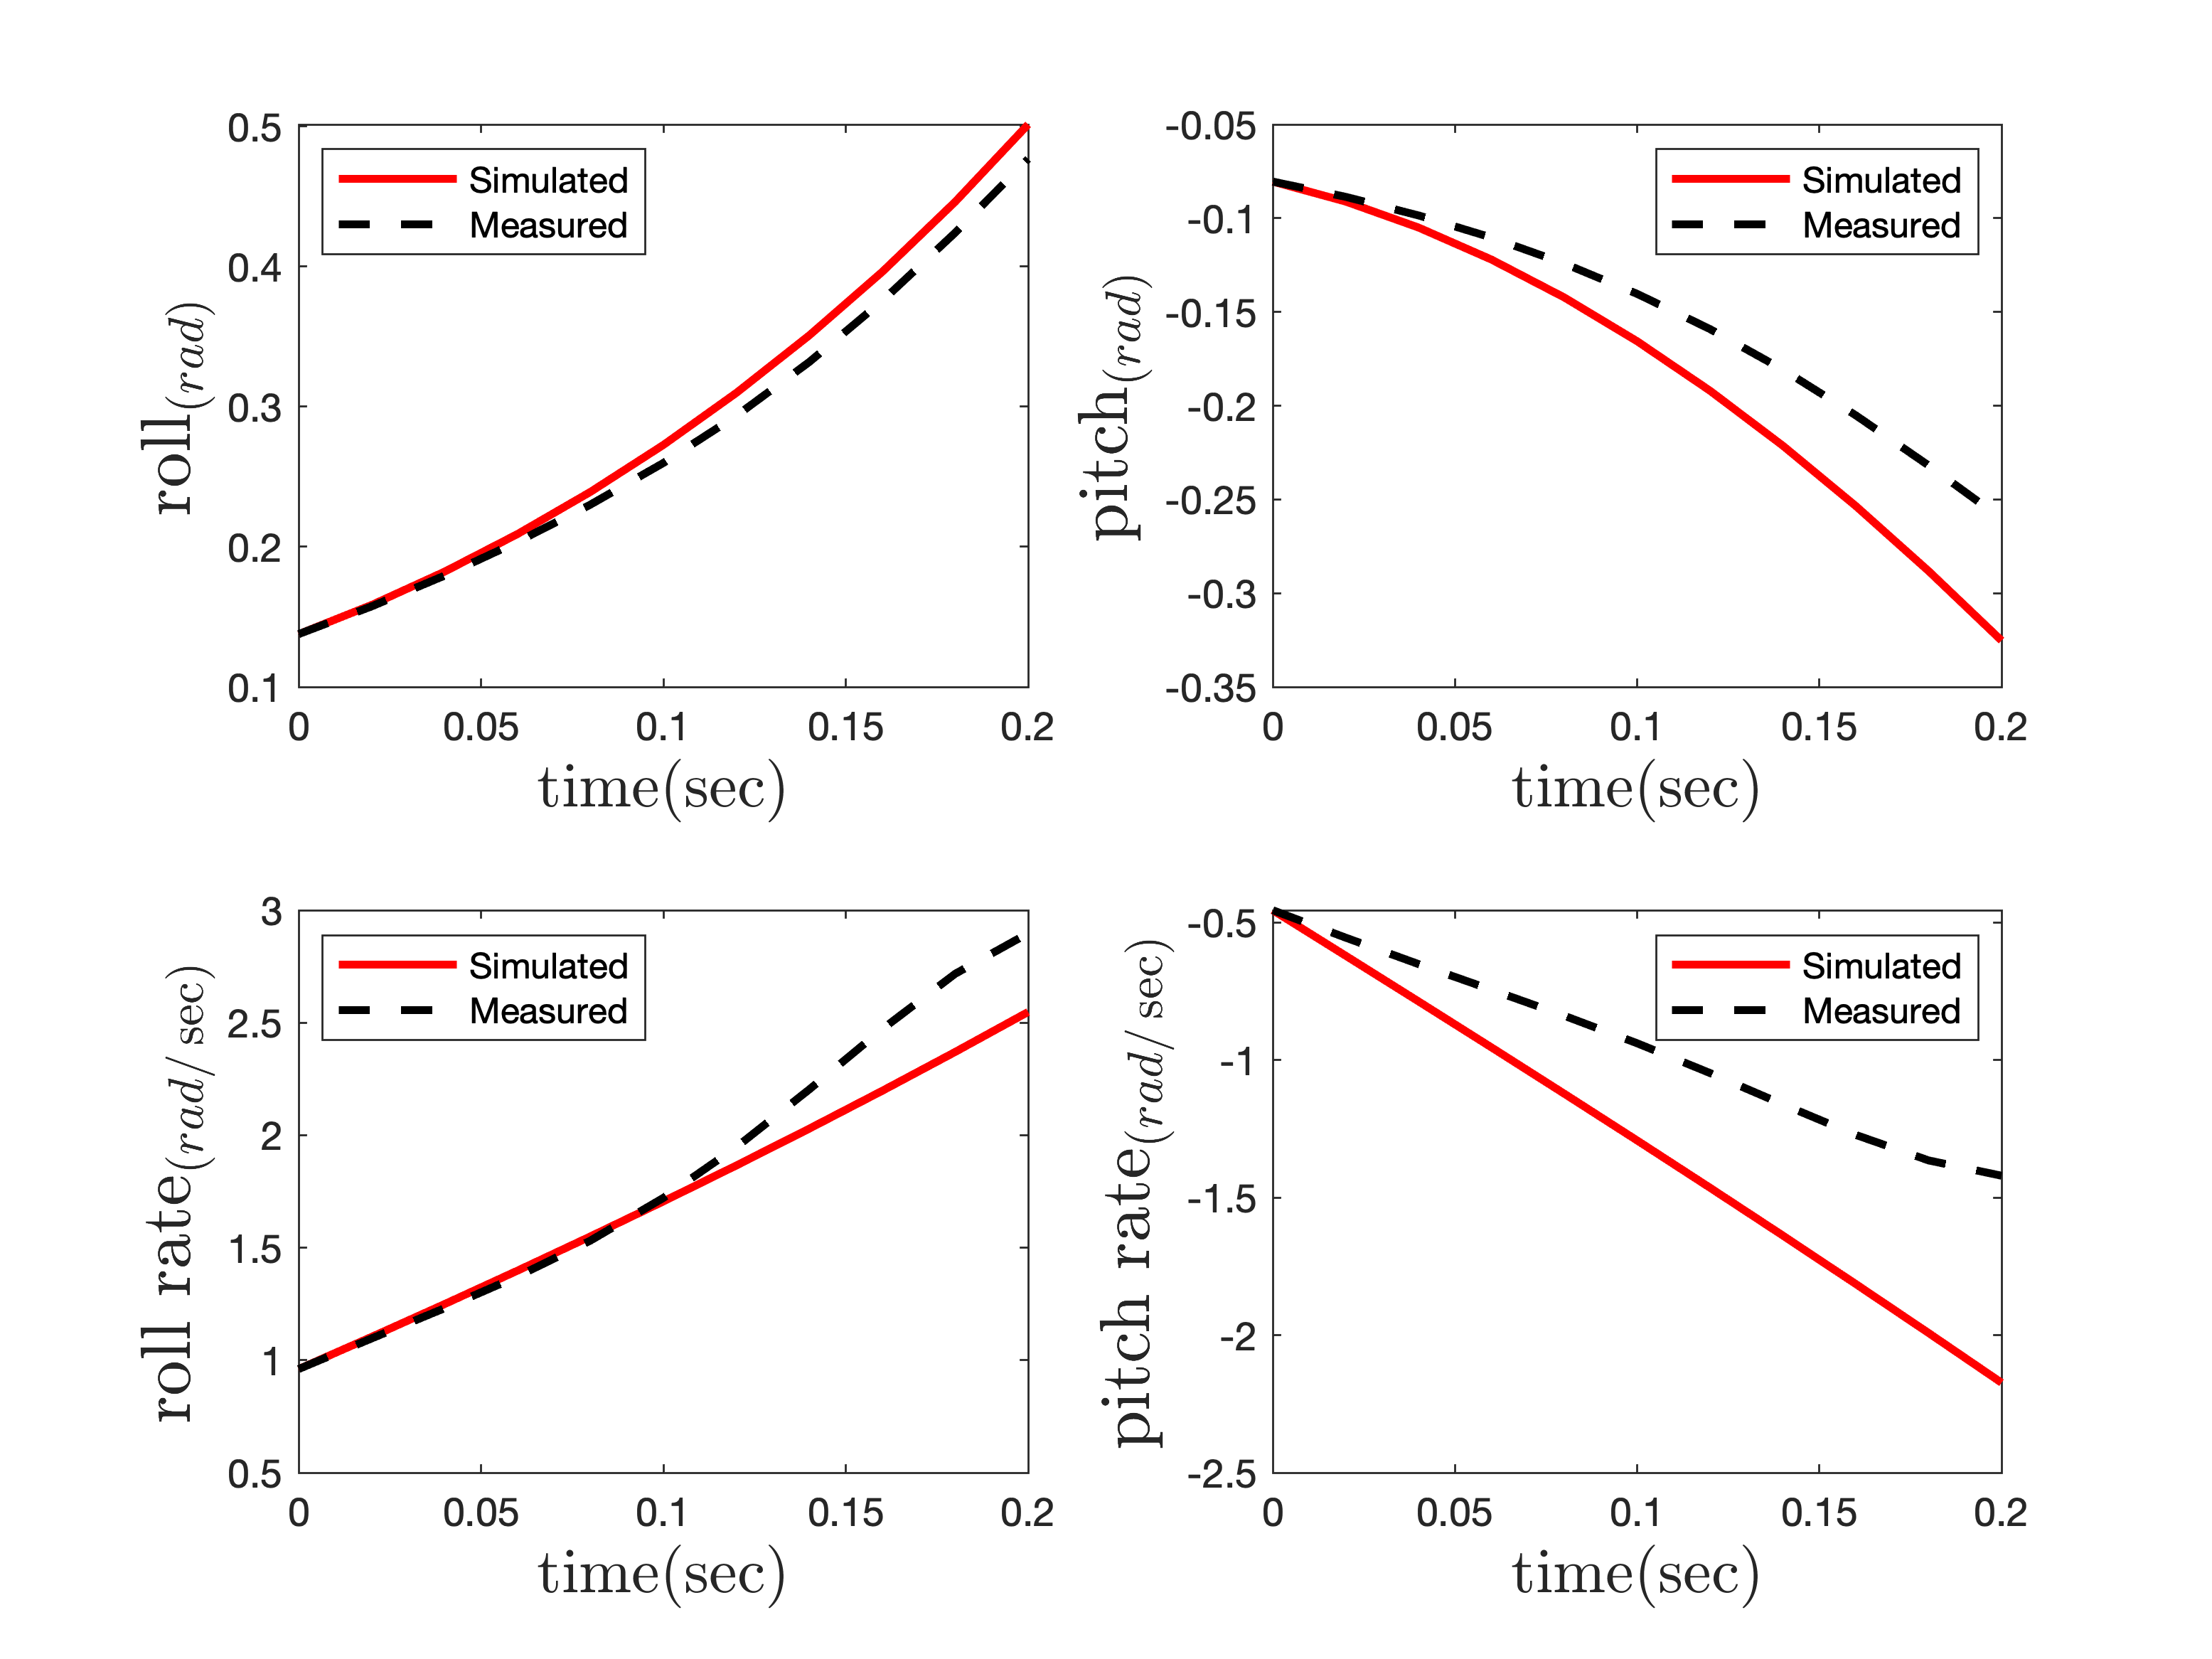
\includegraphics[width=12cm]{../../Figures/RCP/roll_pitch_parameter_estimation/RCP_roll_pitch_S4.png}
	\centering
	\caption{مقايسه خروجی‌های آزمايش چهارم و خروجی‌های شبیه‌سازی پس از تخمین پارامترهای کانال‌های رول-پیچ}
	\label{roll_pitch_ps4}
\end{figure}
\begin{figure}[H]
	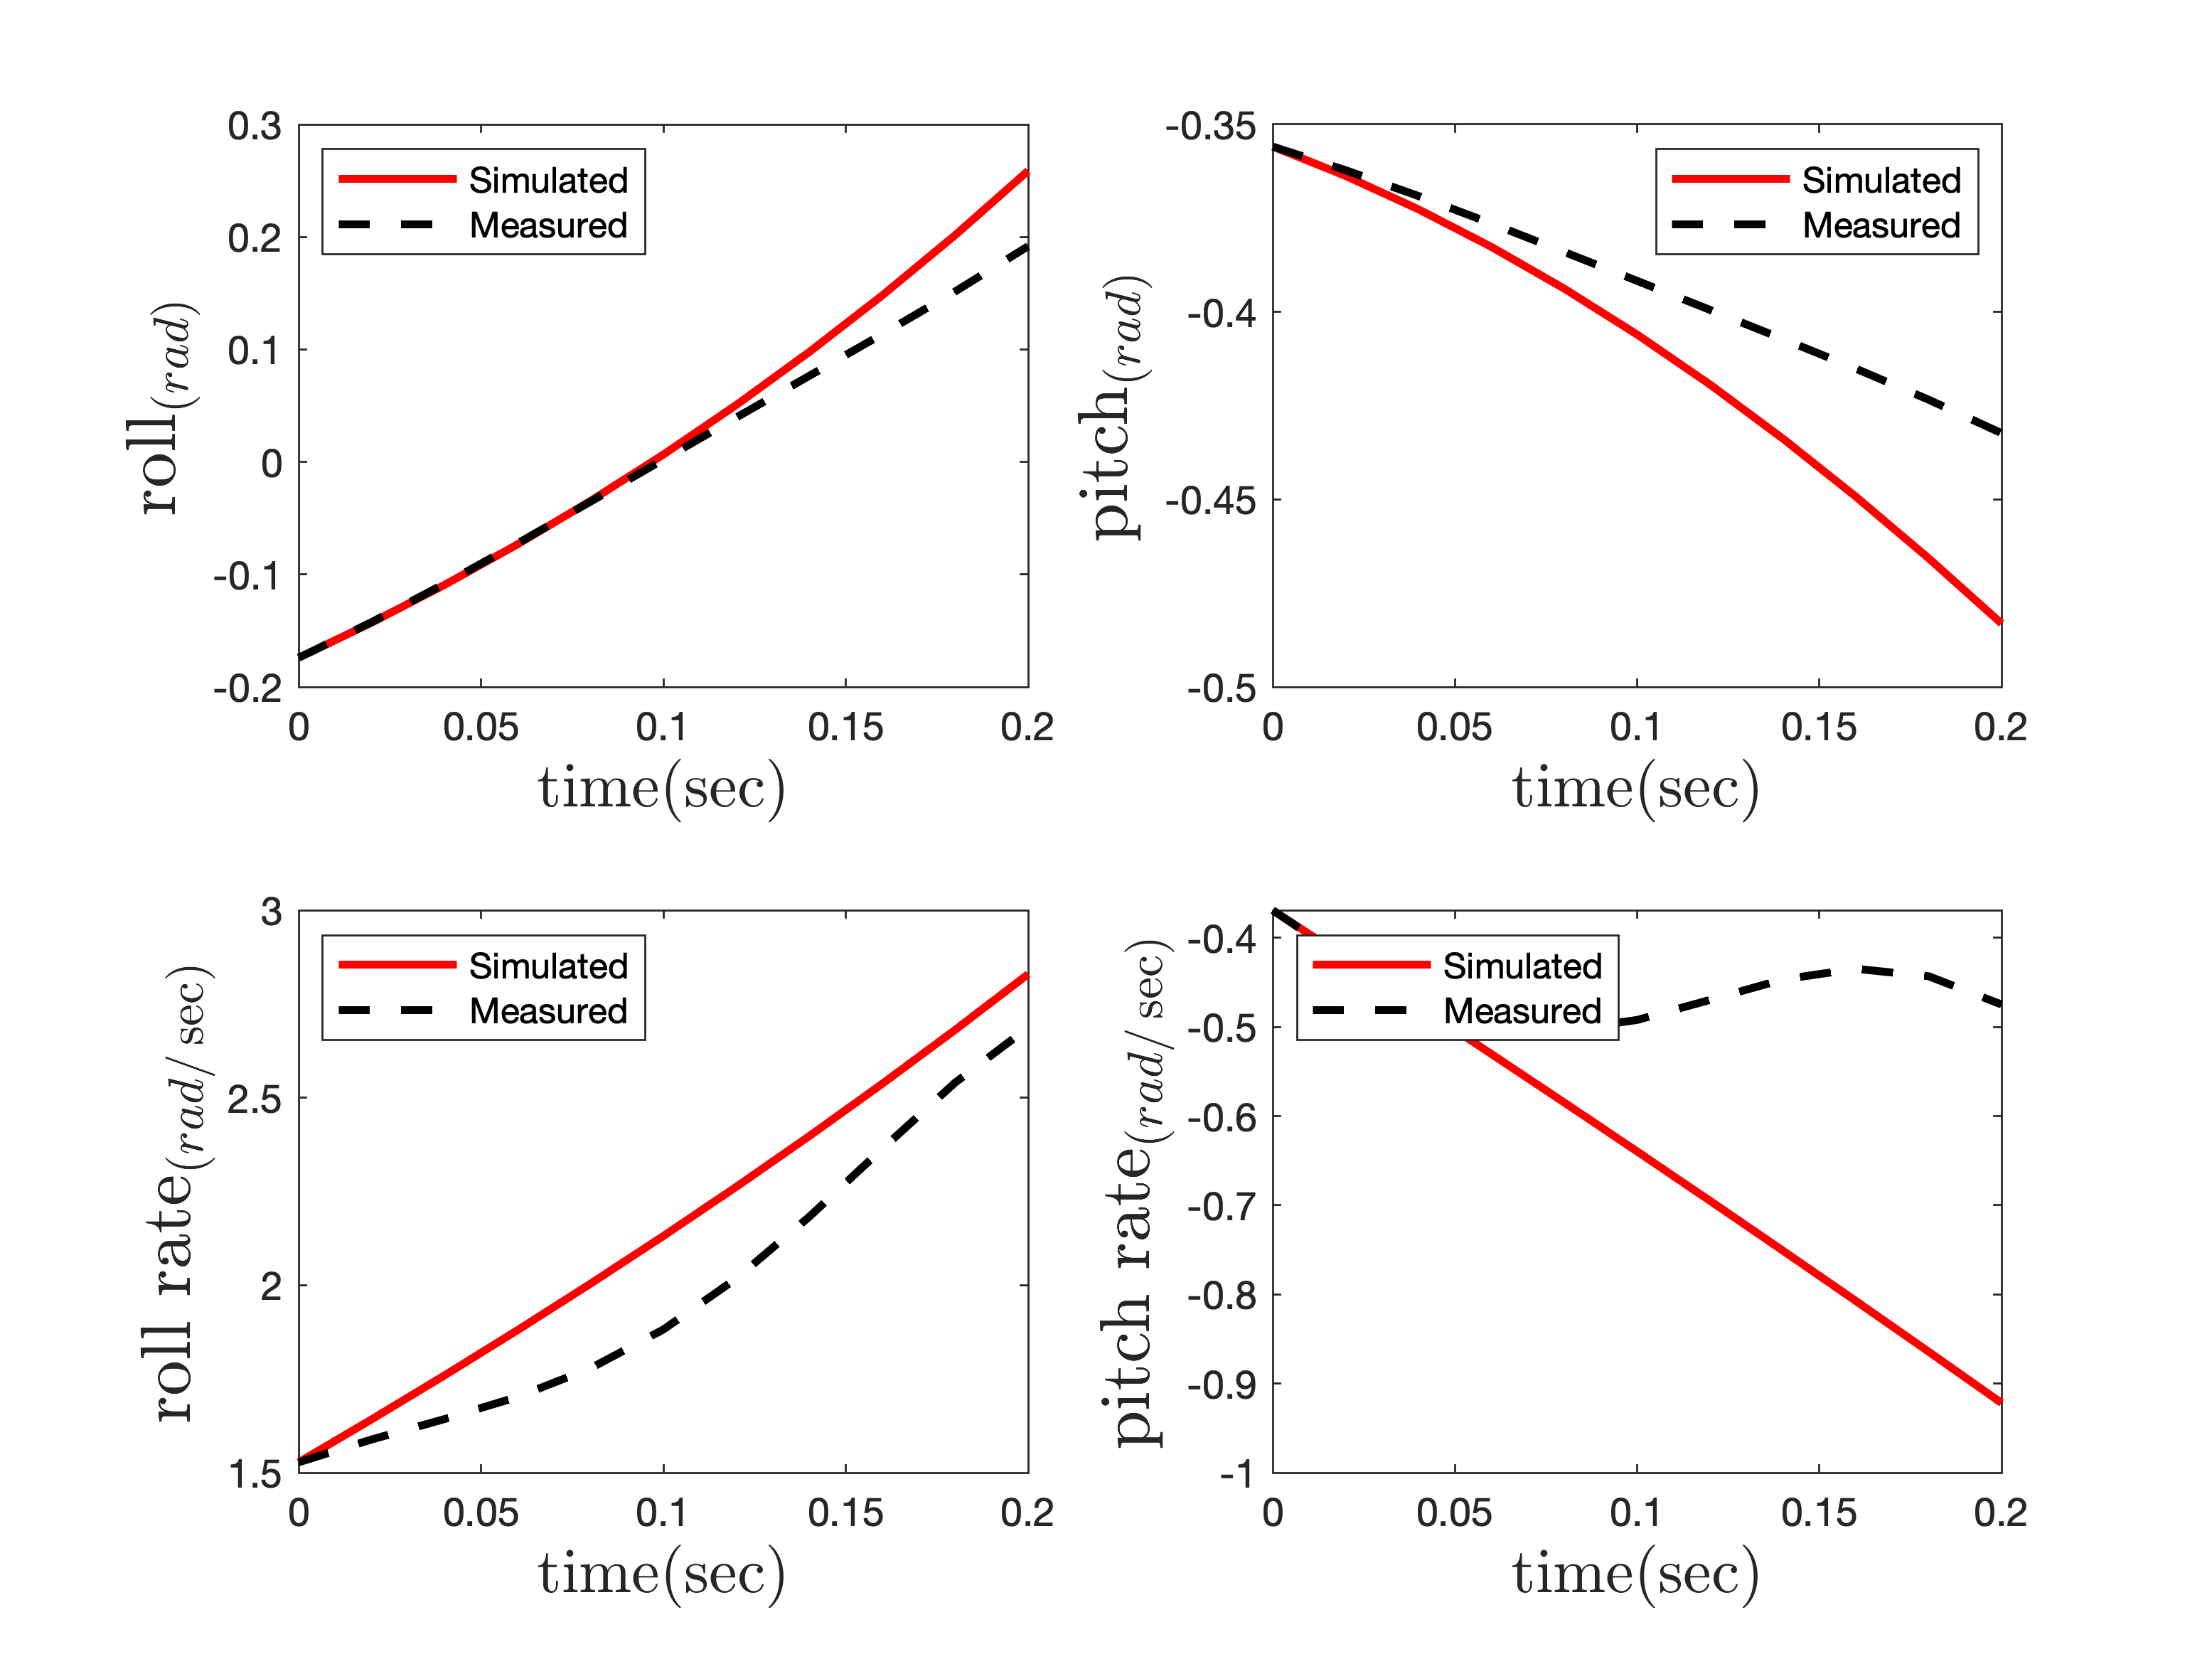
\includegraphics[width=12cm]{../../Figures/RCP/roll_pitch_parameter_estimation/RCP_roll_pitch_S5.png}
	\centering
	\caption{مقايسه خروجی‌های آزمايش پنجم و خروجی‌های شبیه‌سازی پس از تخمین پارامترها کانال‌های رول-پیچ}
	\label{roll_pitch_ps5}
\end{figure}
\begin{figure}[H]
	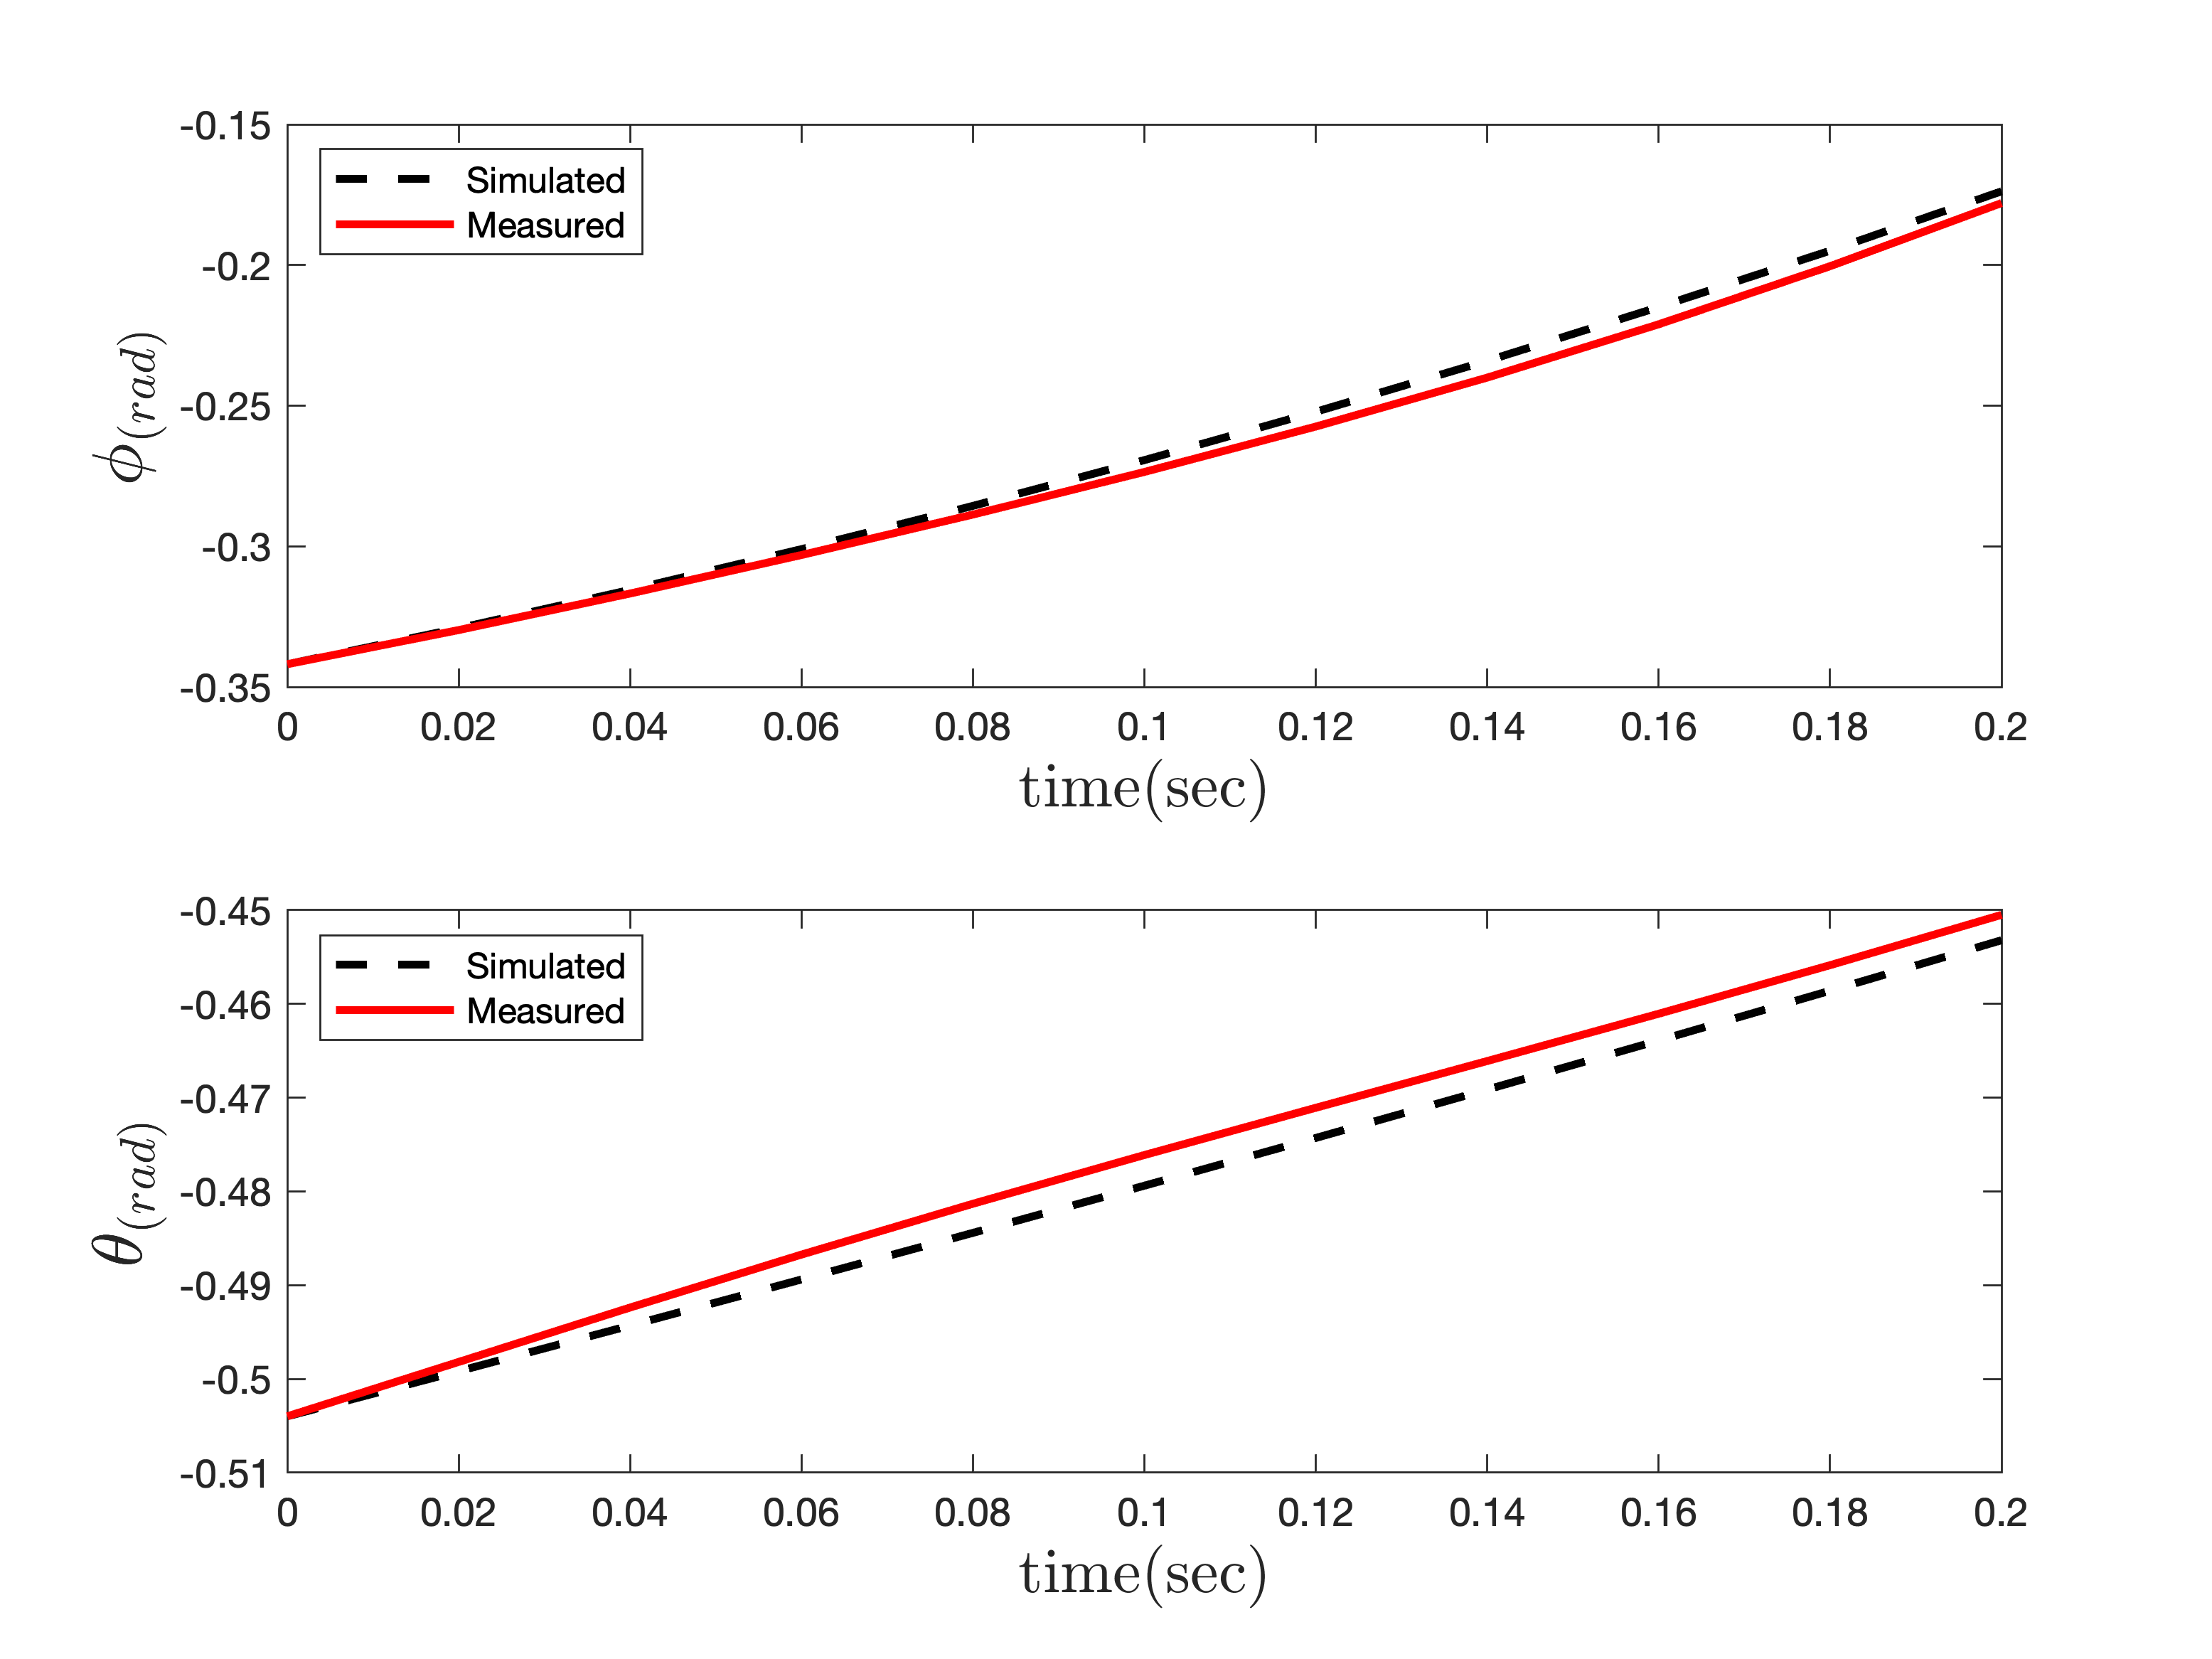
\includegraphics[width=12cm]{../../Figures/RCP/roll_pitch_parameter_estimation/RCP_roll_pitch_S6.png}
	\centering
	\caption{مقايسه خروجی‌های آزمايش ششم و خروجی‌های شبیه‌سازی پس از تخمین پارامترها کانال‌های رول-پیچ}
	\label{roll_pitch_ps6}
\end{figure}
\begin{figure}[H]
	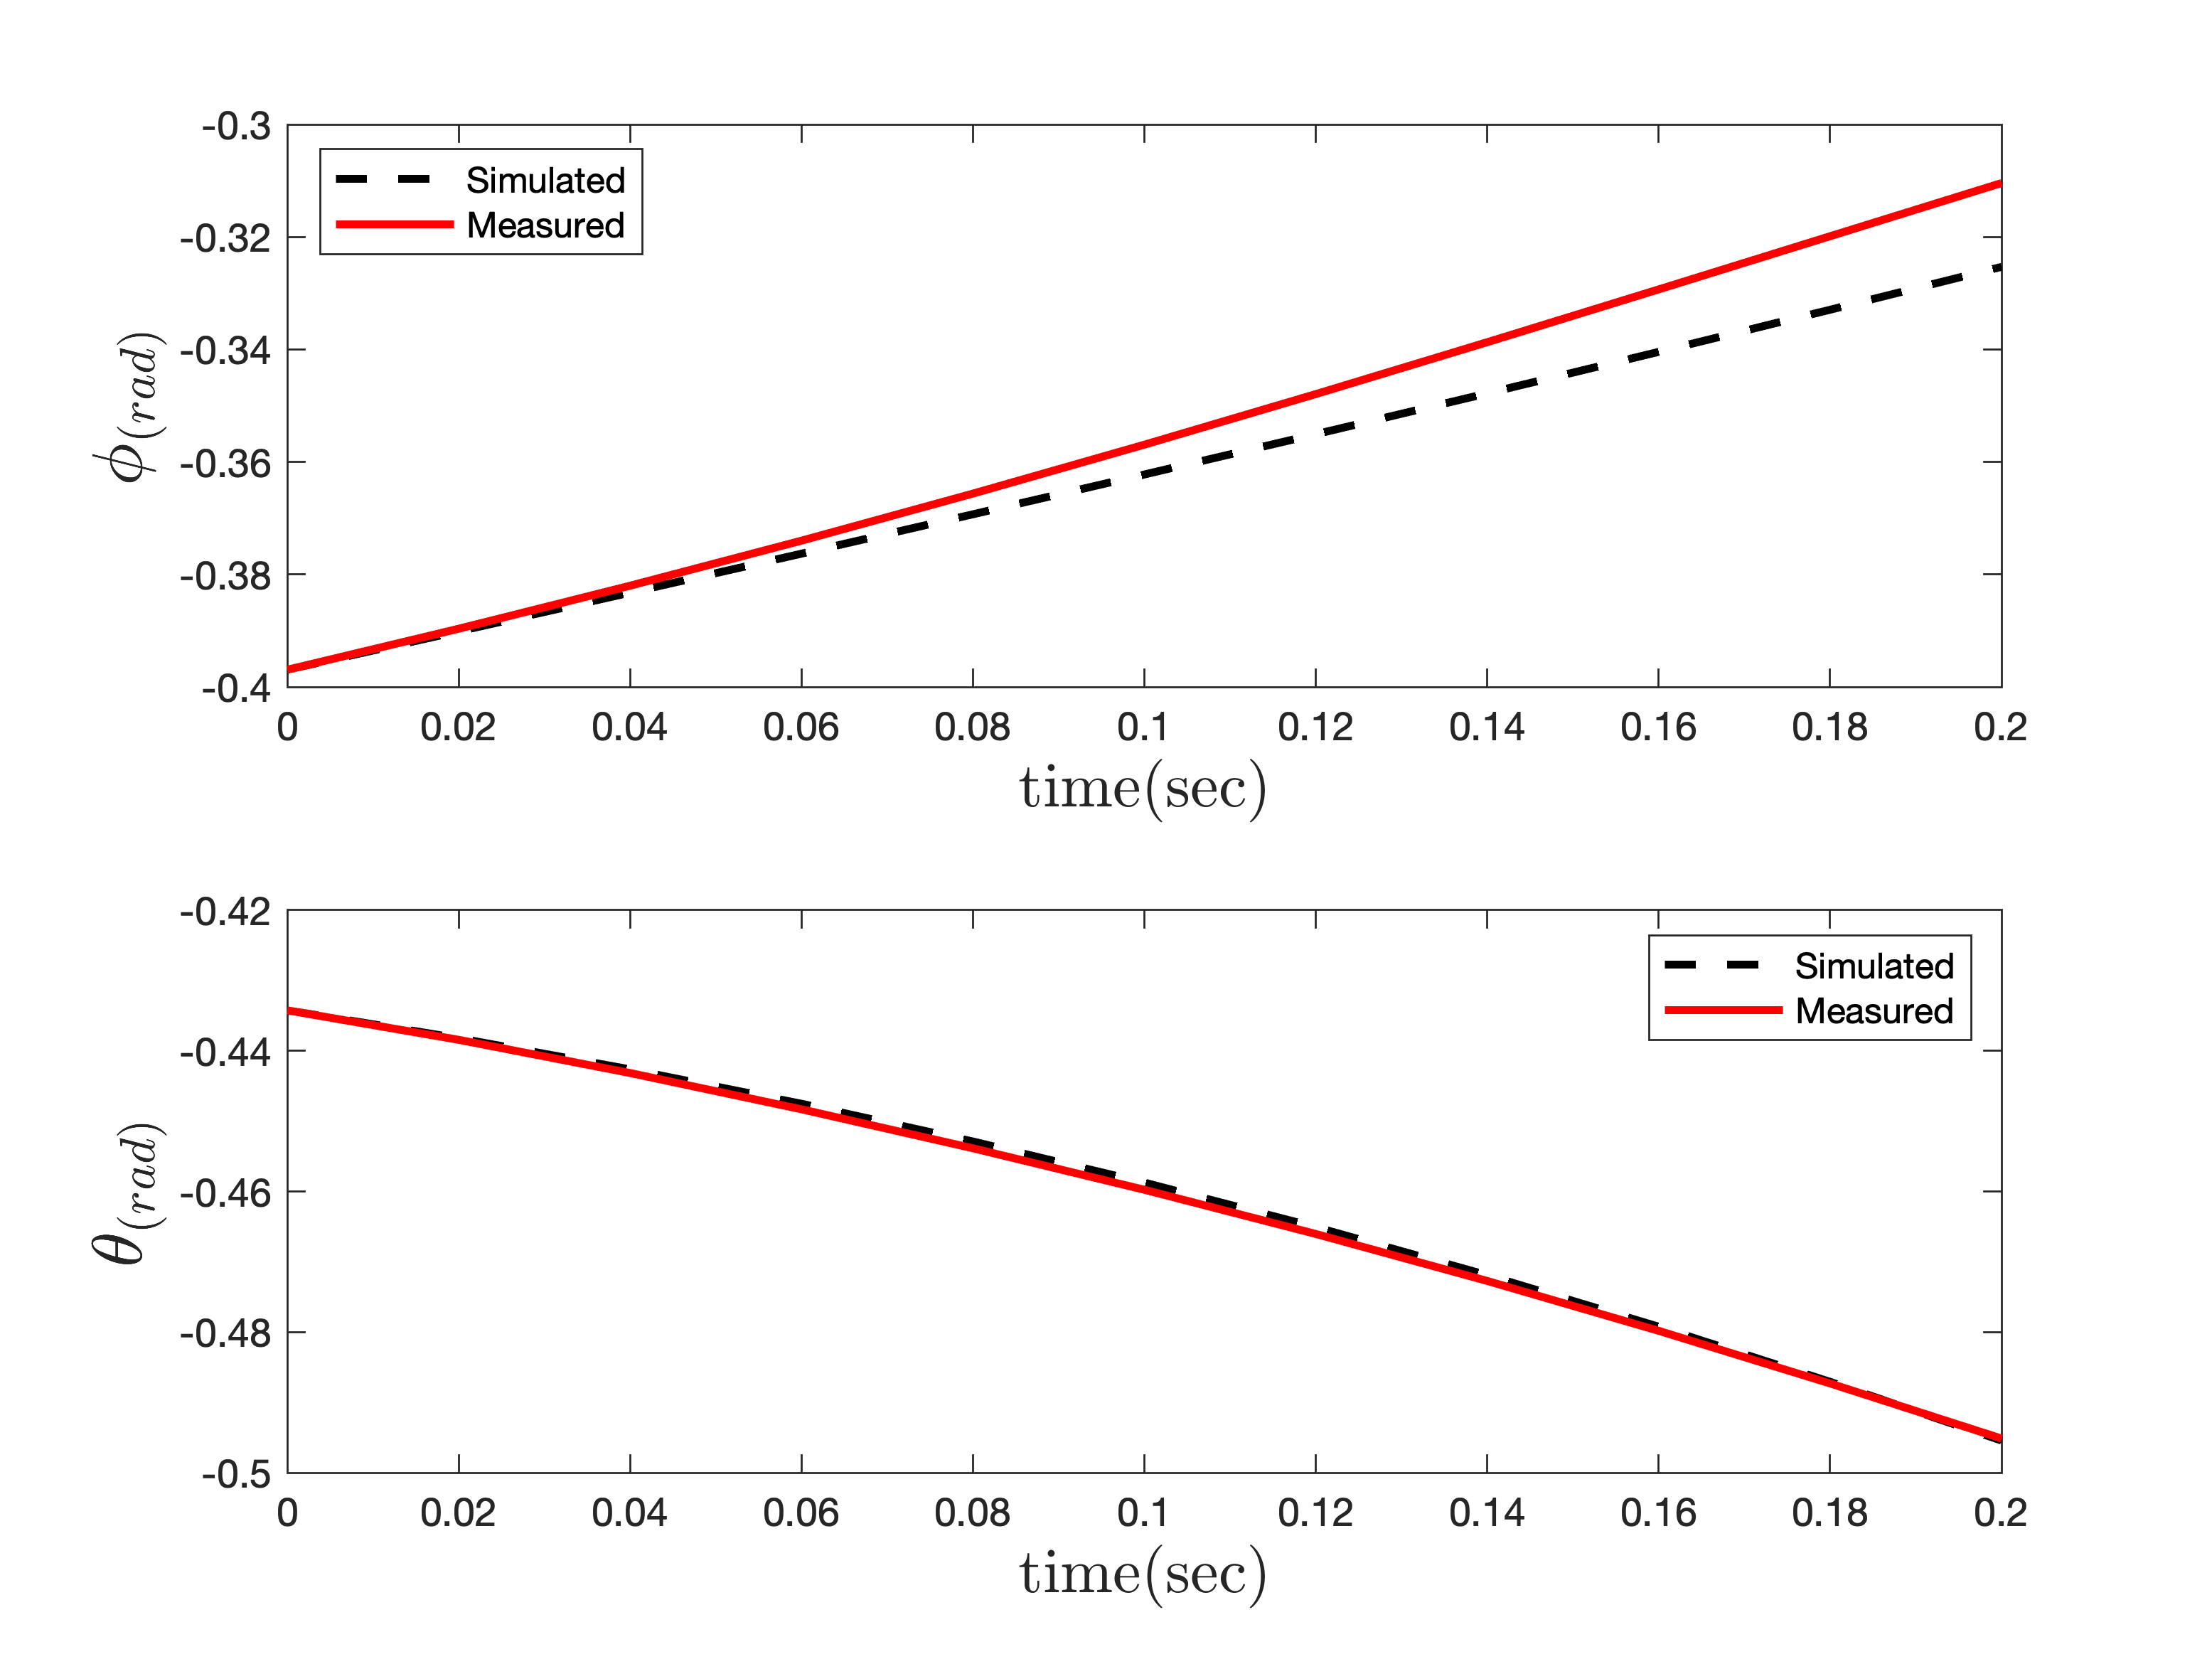
\includegraphics[width=12cm]{../../Figures/RCP/roll_pitch_parameter_estimation/RCP_roll_pitch_S7.png}
	\centering
	\caption{مقايسه خروجی‌های آزمايش هفتم و خروجی‌های شبیه‌سازی پس از تخمین پارامترها کانال‌های رول-پیچ}
	\label{roll_pitch_ps7}
\end{figure}